%%%%%%%%%%%%%%%%%%%%%%%%%%%%%%%%%%%%%%%%%%%%%%%%%%%%%%%%%%%%%%%%%%%%%%%%%%%%%%
% CS110: Introduction to Computing
% Copyright 2015 Pejman Ghorbanzade <mail@ghorbanzade.com>
% Creative Commons Attribution-ShareAlike 4.0 International License
% https://github.com/ghorbanzade/UMB-CS110-2015S/blob/master/LICENSE
%%%%%%%%%%%%%%%%%%%%%%%%%%%%%%%%%%%%%%%%%%%%%%%%%%%%%%%%%%%%%%%%%%%%%%%%%%%%%%

\def \topDirectory {.}
\def \texDirectory {\topDirectory/src/main/tex}

\documentclass[12pt,letterpaper,twoside]{article}
\usepackage{\texDirectory/template/style/directives}
\usepackage{\texDirectory/template/style/assignment}
%%%%%%%%%%%%%%%%%%%%%%%%%%%%%%%%%%%%%%%%%%%%%%%%%%%%%%%%%%%%%%%%%%%%%%%%%%%%%%
% CS110: Introduction to Computing
% Copyright 2015 Pejman Ghorbanzade <mail@ghorbanzade.com>
% Creative Commons Attribution-ShareAlike 4.0 International License
% https://github.com/ghorbanzade/UMB-CS110-2015S/blob/master/LICENSE
%%%%%%%%%%%%%%%%%%%%%%%%%%%%%%%%%%%%%%%%%%%%%%%%%%%%%%%%%%%%%%%%%%%%%%%%%%%%%%

\course{id}{CS110}
\course{name}{Introduction to Computing}
\course{venue}{Tue/Thu, 5:30 PM - 6:45 PM}
\course{semester}{Spring 2015}
\course{department}{Department of Computer Science}
\course{university}{University of Massachusetts Boston}

\instructor{name}{Pejman Ghorbanzade}
\instructor{title}{}
\instructor{position}{Student Instructor}
\instructor{email}{pejman@cs.umb.edu}
\instructor{phone}{617-287-6419}
\instructor{office}{S-3-124B}
\instructor{office-hours}{Tue/Thu 19:00-20:30}
\instructor{address}{University of Massachusetts Boston, 100 Morrissey Blvd., Boston, MA}


\begin{document}

\doc{title}{Assignment 1}
\doc{date-pub}{Feb 03, 2015 at 5:30 PM}
\doc{date-due}{Feb 17, 2015 at 5:30 PM}
\doc{points}{8}

\prepare{header}

\section*{Question 1}

The code snippet below gives a Java \textit{Hello World!} program.
\lstset{language=Java}
\begin{lstlisting}
public class HelloJava {
	public static void main(String[] args) {
		System.out.println("Hello World!");
	}
}
\end{lstlisting}
As we discussed in class, Java is not the only programming language capable of such miracles. Write programs \texttt{HelloPython.py}, \texttt{HelloC.c} and \texttt{HelloPhp.php} that print \textit{Hello World!} in Python, C and Php programming languages, respectively.
\begin{figure}[H]\centering
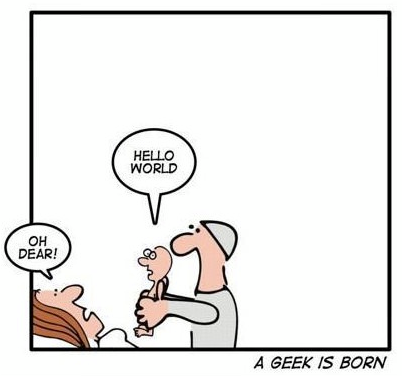
\includegraphics[width=8cm]{\texDirectory/template/images/helloworld.png}
\end{figure}

\section*{Question 2}

Generally, a programmer's objective is to develop a program with no \textit{compilation error} that functions as originally desired, i.e. no \textit{run-time error}.
But errors occur almost inevitably during development of any program.
A reliable measure of a programmer's proficiency is how efficiently he can identify and fix his errors.
To do this, however, one must first understand the errors.

In this question, you are asked to intentionally introduce compilation-errors to your \texttt{HelloWorld.java} program. Prepare a file \texttt{ErrorList.txt}, listing as many different compiler complaints as possible along with mistake(s) which cause them.

\section*{Question 3}

Write a program \texttt{Cartesian.java} that takes three command-line arguments as $X$, $Y$ and $Z$ in Cartesian coordinates and prints their corresponding $\rho$, $\theta$ and $\phi$ in Spherical coordinates.

\section*{Question 4}

Write a program \texttt{BodyMassIndex.java} that takes your weight in pounds and height in inches and calculates your Body Mass Index (BMI) according to Equation \ref{eq1}. To evaluate your BMI, program should as well indicate under which group you are classified according to Table \ref{tab1} obtained from the Department of Health and Human Services/National Institution of Health.
\begin{equation}
BMI = \frac{weightInPounds \times 703}{heightInInches^2}
\label{eq1}
\end{equation}
\begin{table}[H]\centering
\begin{tabular}{|r|l|}
\hline
Group & BMI index \\
\hline
Underweight & less than 18.5 \\
Normal & between 18.5 and 24.9 \\
Overweight & between 25 and 29.9 \\
Obese & greater than or equal to 30 \\
\hline
\end{tabular}
\caption{BMI classification}\label{tab1}
\end{table}
\newpage

\section*{Question 5}

Write a program \texttt{Quadratic.java} that takes three integers $a$, $b$ and $c$ as command-line arguments and solves for $x$ with three digits of precision, the quadratic expression shown in Equation \ref{eq2}.
\begin{equation}
ax^2+bx+c=0
\label{eq2}
\end{equation}
Note that when discriminant is not negative, root(s) of a quadratic equation are obtained from Equation \ref{eq3}. When discriminant is negative, however, no real solution exists.
\begin{equation}
x = \frac{-b \pm \sqrt[2]{b^2-4ac}}{2a}
\label{eq3}
\end{equation}
Your program is expected to function as shown in following examples.

\textbf{Example:}
\begin{verbatim}
% java Quadratic 1 -2 -4
Solutions are -1.236 and 3.237
% java Quadratic 9 12 4
Solution is -0.667
% java Quadratic 3 4 2
No real-number solution exists
\end{verbatim}

\prepare{footer}

\end{document}
